\chapter{Lay Summary}
\epigraph{“With magic, you can turn a frog into a prince. With science, you can turn a frog into a Ph.D and you still have the frog you started with.”}{Terry Pratchett}

\begin{wrapfigure}{r}{0.4\textwidth}
\centering
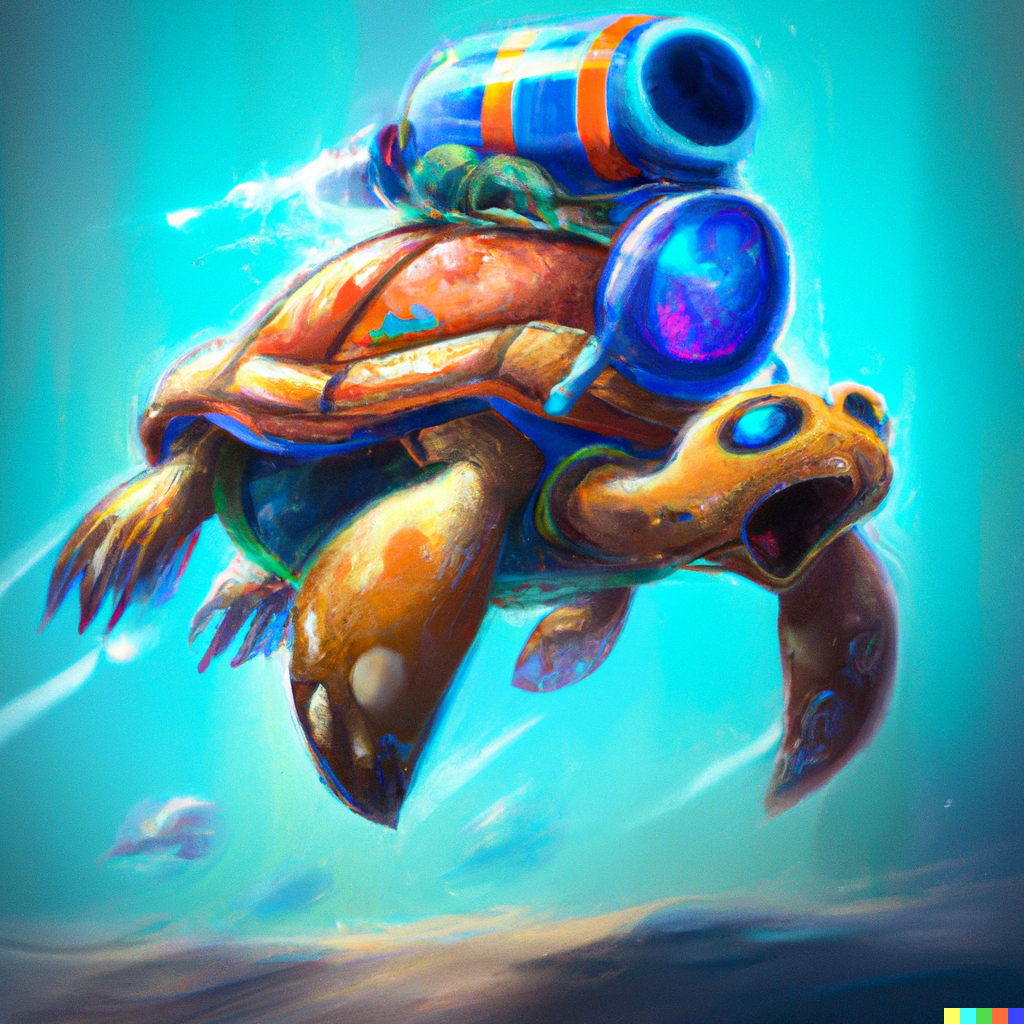
\includegraphics[width=0.9\linewidth]{images/COLD_turle.png} \caption[DALL$\cdot$E turtle illustration.]{A turtle with a jetpack strapped to its back, illustrating the speed-up of what is canonically a slow (adiabatic) process. This image was created with the assistance of DALL$\cdot$E 2 \cite{noauthor_dalle_nodate}.}\label{fig:COLD_TURTLE}
\vspace{-5pt}
\end{wrapfigure}

Quantum systems are notoriously volatile creatures. In our quest to build better quantum technologies, we must first learn the art of \emph{controlling} them with very high precision in a way that produces useful information or work. This must be done while protecting the information such systems contain from an environment that is often hell-bent on making this job as difficult as possible \footnote{This anthropomorphisation of quantum systems and the environment is for literary effect - I do not believe that the environment has much in the way of a political agenda to inflict decoherence upon quantum systems}.

A particularly useful type of controlled process that we would like to be able to perform is an \emph{adiabatic} process, which involves slowly changing some parameter affecting a quantum system, \@e.g.~the strength or direction of an electromagnetic field. The `slow' part here is required to keep the system from getting excited out of the `instantaneous' energy level that it starts in. Think of slowly rotating a magnetic field such that a magnet always stays aligned with the field. If the change happens too quickly, the magnet overshoots in the direction of the changing field. An analogous process happens in the quantum case, where the quantum state `jumps' out of its energy level. For many applications of quantum technologies, we would like to avoid such jumps, hence we perform adiabatic (slow) transformations.

Unfortunately, the volatility of quantum systems does not often allow us to abide by this slow condition. The longer a quantum process takes to complete, the more time it spends exposed to the environment, leaking information and absorbing heat. In order to combat this lossiness, entire fields of study have been developed with the sole aim of imitating the results of adiabatic processes on shorter timescales. The techniques used to achieve this vary vastly and achieve various levels of success: some suppress the losses that come with fast processes, others try to avoid them entirely with increasingly complex protocols.

In this thesis, we present a method which aims to speed up adiabatic processes in a way that caters to the practical constraints of quantum experiments. We assume that we are given a limited set of operations that we can actually perform in order to suppress some of the jumps that occur during fast driving. We then optimise the path through which the system travels in a way that helps this very restricted set of operations perform as best as they could. This approach follows the fact that the losses depend on the path that the system parameter takes: for example, the magnetic field can rotate from its starting direction to the final one while including detours and oscillations along the way, which will all have an impact on the likelihood that some kind of jump happens. If you get that path just right, it is possible to mitigate or suppress many of the effects of a fast change quite efficiently in many cases. We demonstrate this in some of the later chapters with simulations of such optimised counterdiabatic protocols for different systems and different rates of change in the system parameters. 

For more details, I invite you to read my blog post on the topic given by Ref. \cite{cepaite_cold_2023}, which is slightly more technical and detailed, but brief and full of animations to explain the concepts involved. 
